\documentclass[../main.tex]{subfiles}

\begin{document}

\subsection{Resultados: Promedio de 10 experimentos}

Pues se ve similar a la gŕafica anterior.

\begin{figure}[ht!]
    \centering
    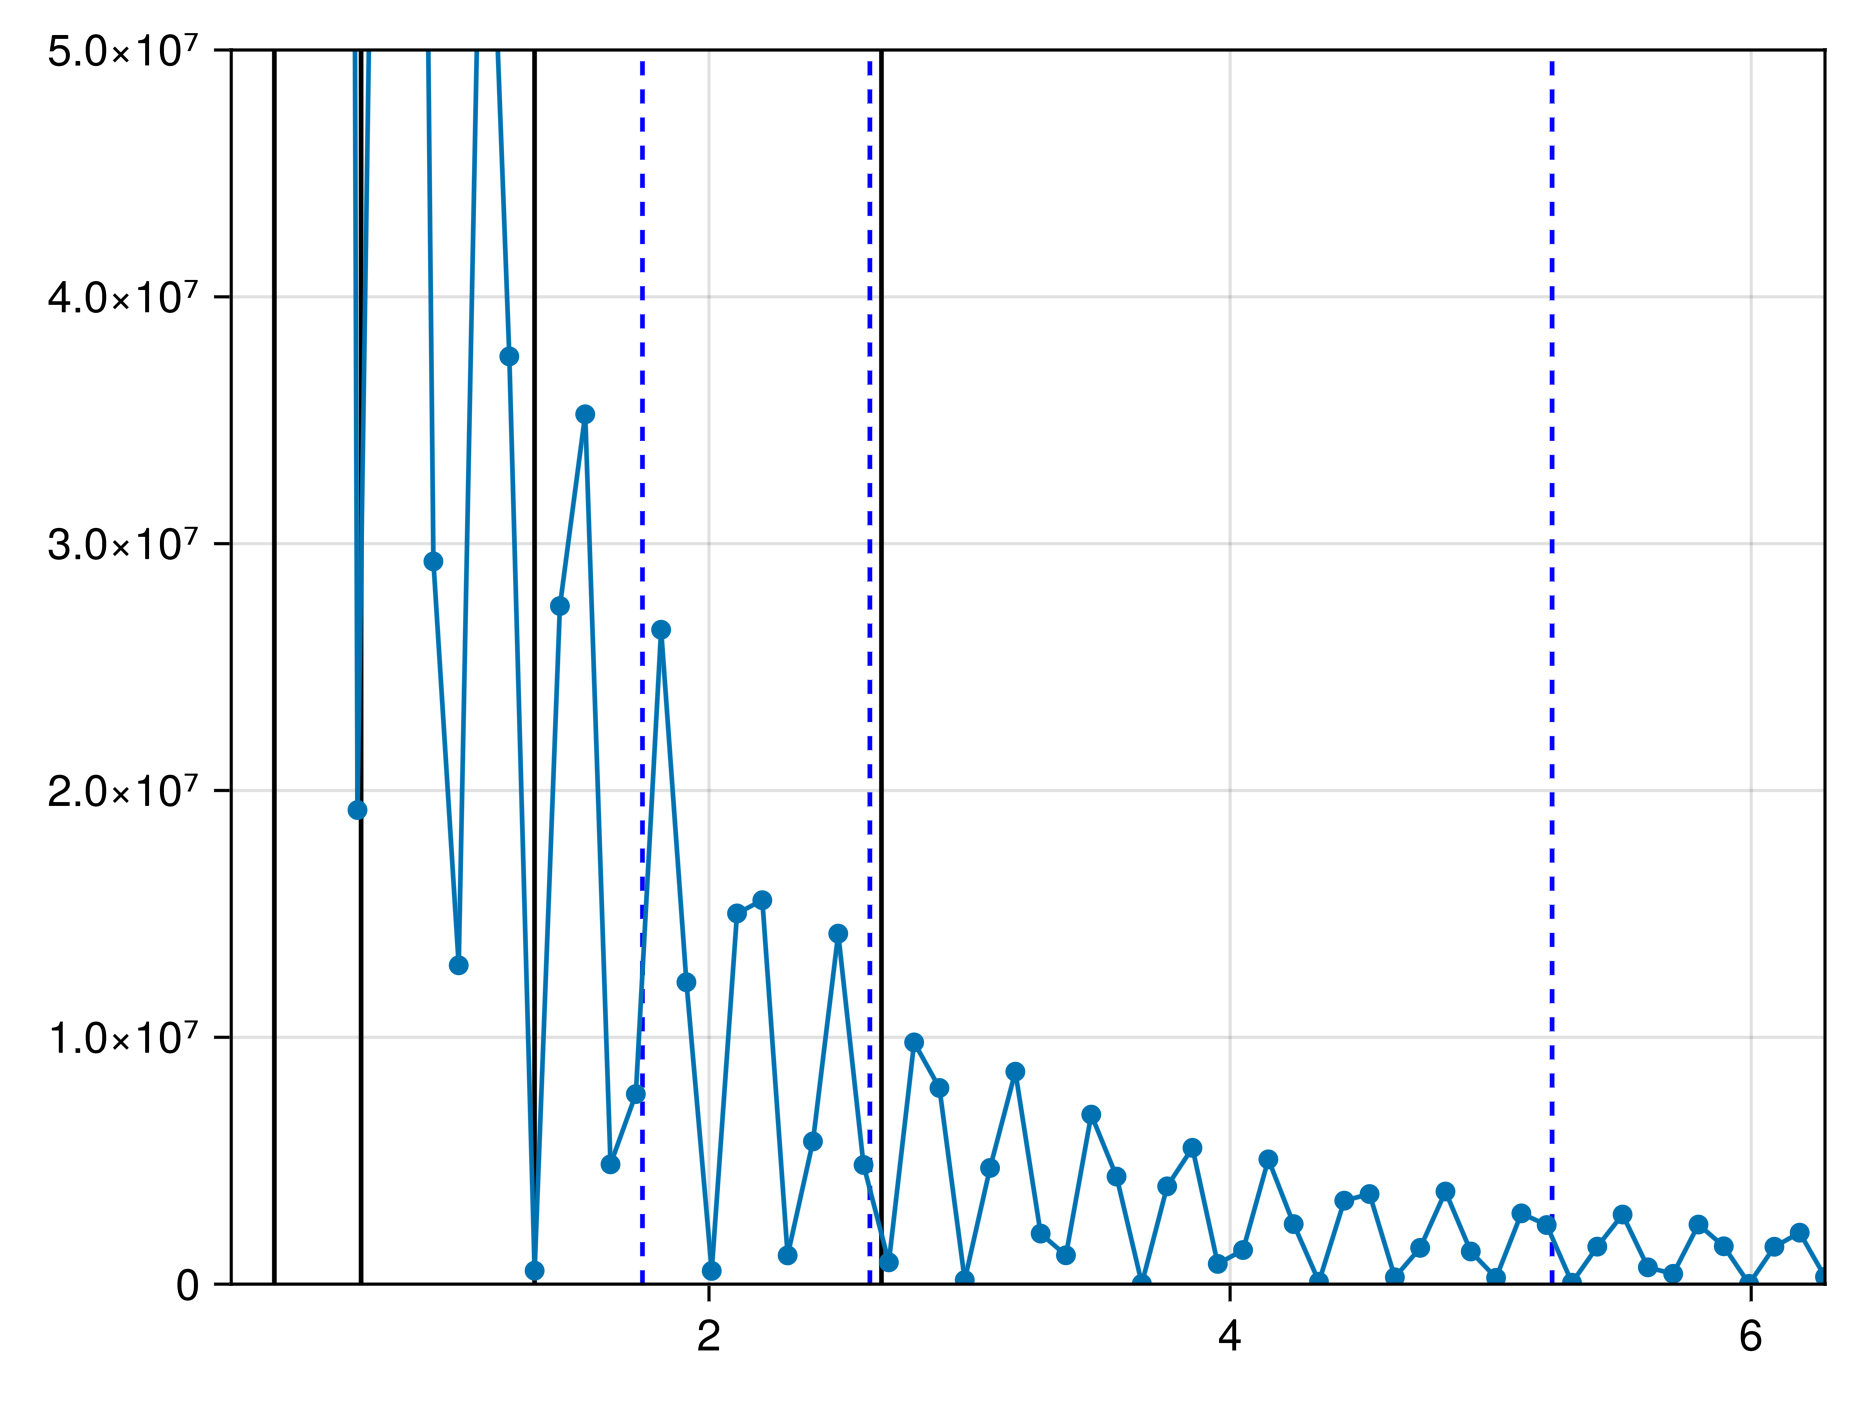
\includegraphics[width=0.9\textwidth]{../Figures/may8/fig_SqCorreccion3_phi5_d_zoom1_nexp10.png}
    \caption{Factor de estructura con la corrección. \(\phi=5\%\). 
    Las líneas verticales punteadas en azúl están ubicadas en \(|\vec{q}|=2\pi/1.2,~|\vec{q}|=2\pi/(2\cdot1.2),~|\vec{q}|=2\pi/(3\cdot1.2)\).
    Las líneas verticales punteadas en negro están ubicadas en \(|\vec{q}|\in\{2\pi/L,2\pi/L/2,2\pi/L/4,2\pi/L/8,2\pi/L/16\}\).
}
\end{figure}

Ocupo hacer unos experimentos con menos direcciones y hacer que las magnitudes sean múltiplos de la distancia característica.

\section{Sugerencias de Claudia}

Mantener las direcciones aleatorias.
Poner las magnitudes en términos de la resolución.
El dominio de la magnitud sería hasta \(N\) veces la resolución.

Estoy teniendo problemas en definir el dominio de las magnitudes del vector de onda.

\paragraph{Resultados de la implementación de las sugerencias de Claudia.}

Me hace un poco más de sentido, pero regresamos un poco al problema de no encontrar picos en distancias que intuyo que serían características.
La siguiente gŕafica es para el sistema en el último tiempo.

\begin{figure}[ht!]
    \centering
    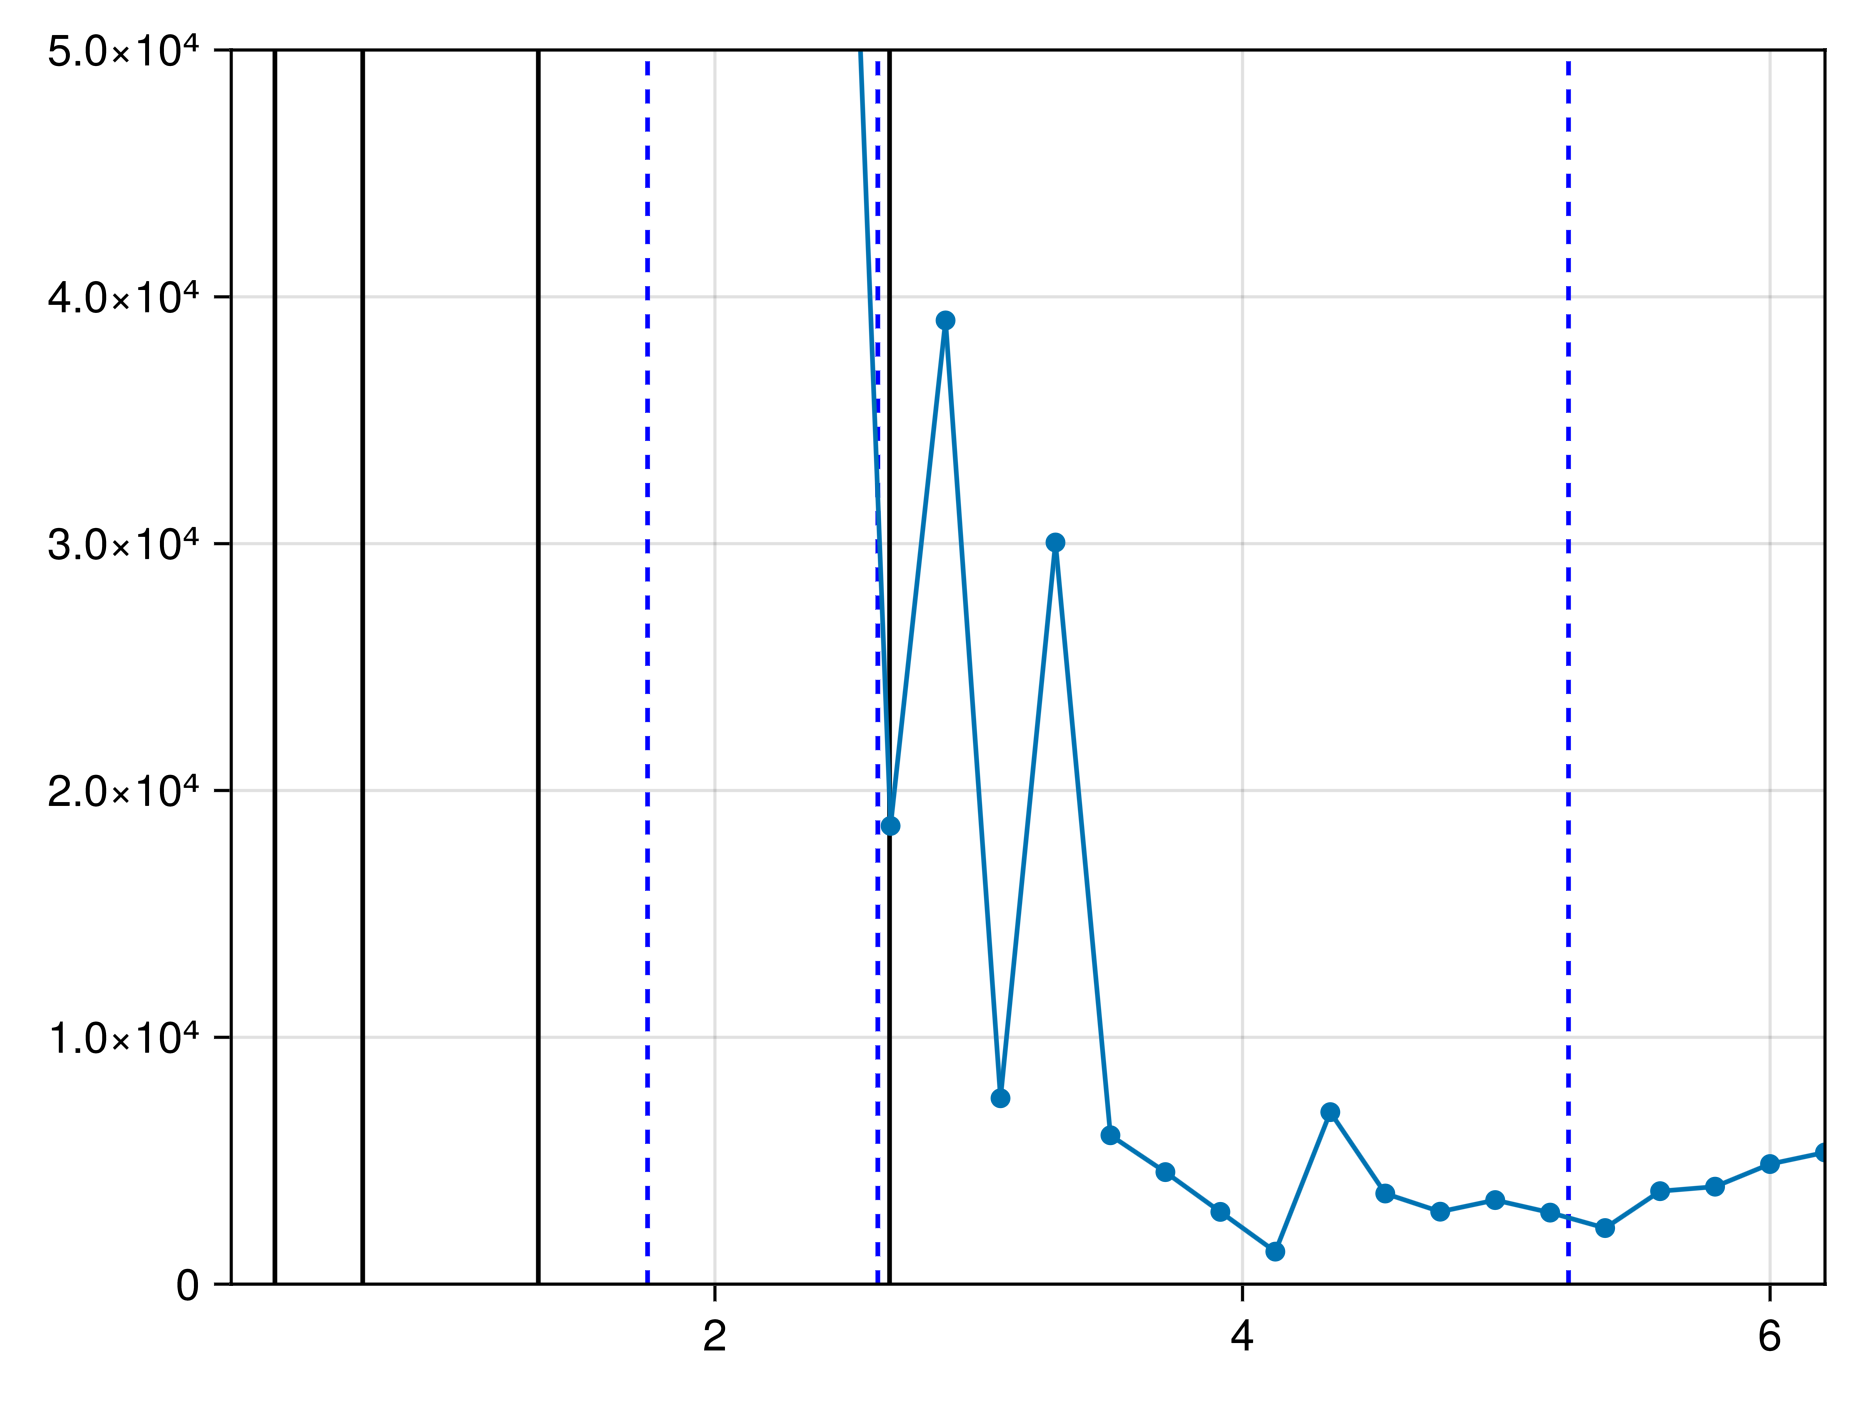
\includegraphics[width=0.9\textwidth]{../Figures/may8/fig_SqCorreccion3A_phi5_d_zoom1_1.png}
    \caption{Tiempo final. 
        Factor de estructura con la corrección. \(\phi=5\%\). 
    Las líneas verticales punteadas en azúl están ubicadas en \(|\vec{q}|=2\pi/1.2,~|\vec{q}|=2\pi/(2\cdot1.2),~|\vec{q}|=2\pi/(3\cdot1.2)\).
    Las líneas verticales punteadas en negro están ubicadas en \(|\vec{q}|\in\{2\pi/L,2\pi/L/2,2\pi/L/4,2\pi/L/8,2\pi/L/16\}\).
}
\end{figure}

La siguiente gráfica es para eltiempo inicial de la simulación, pero no hay mucha diferencia.

\begin{figure}[ht!]
    \centering
    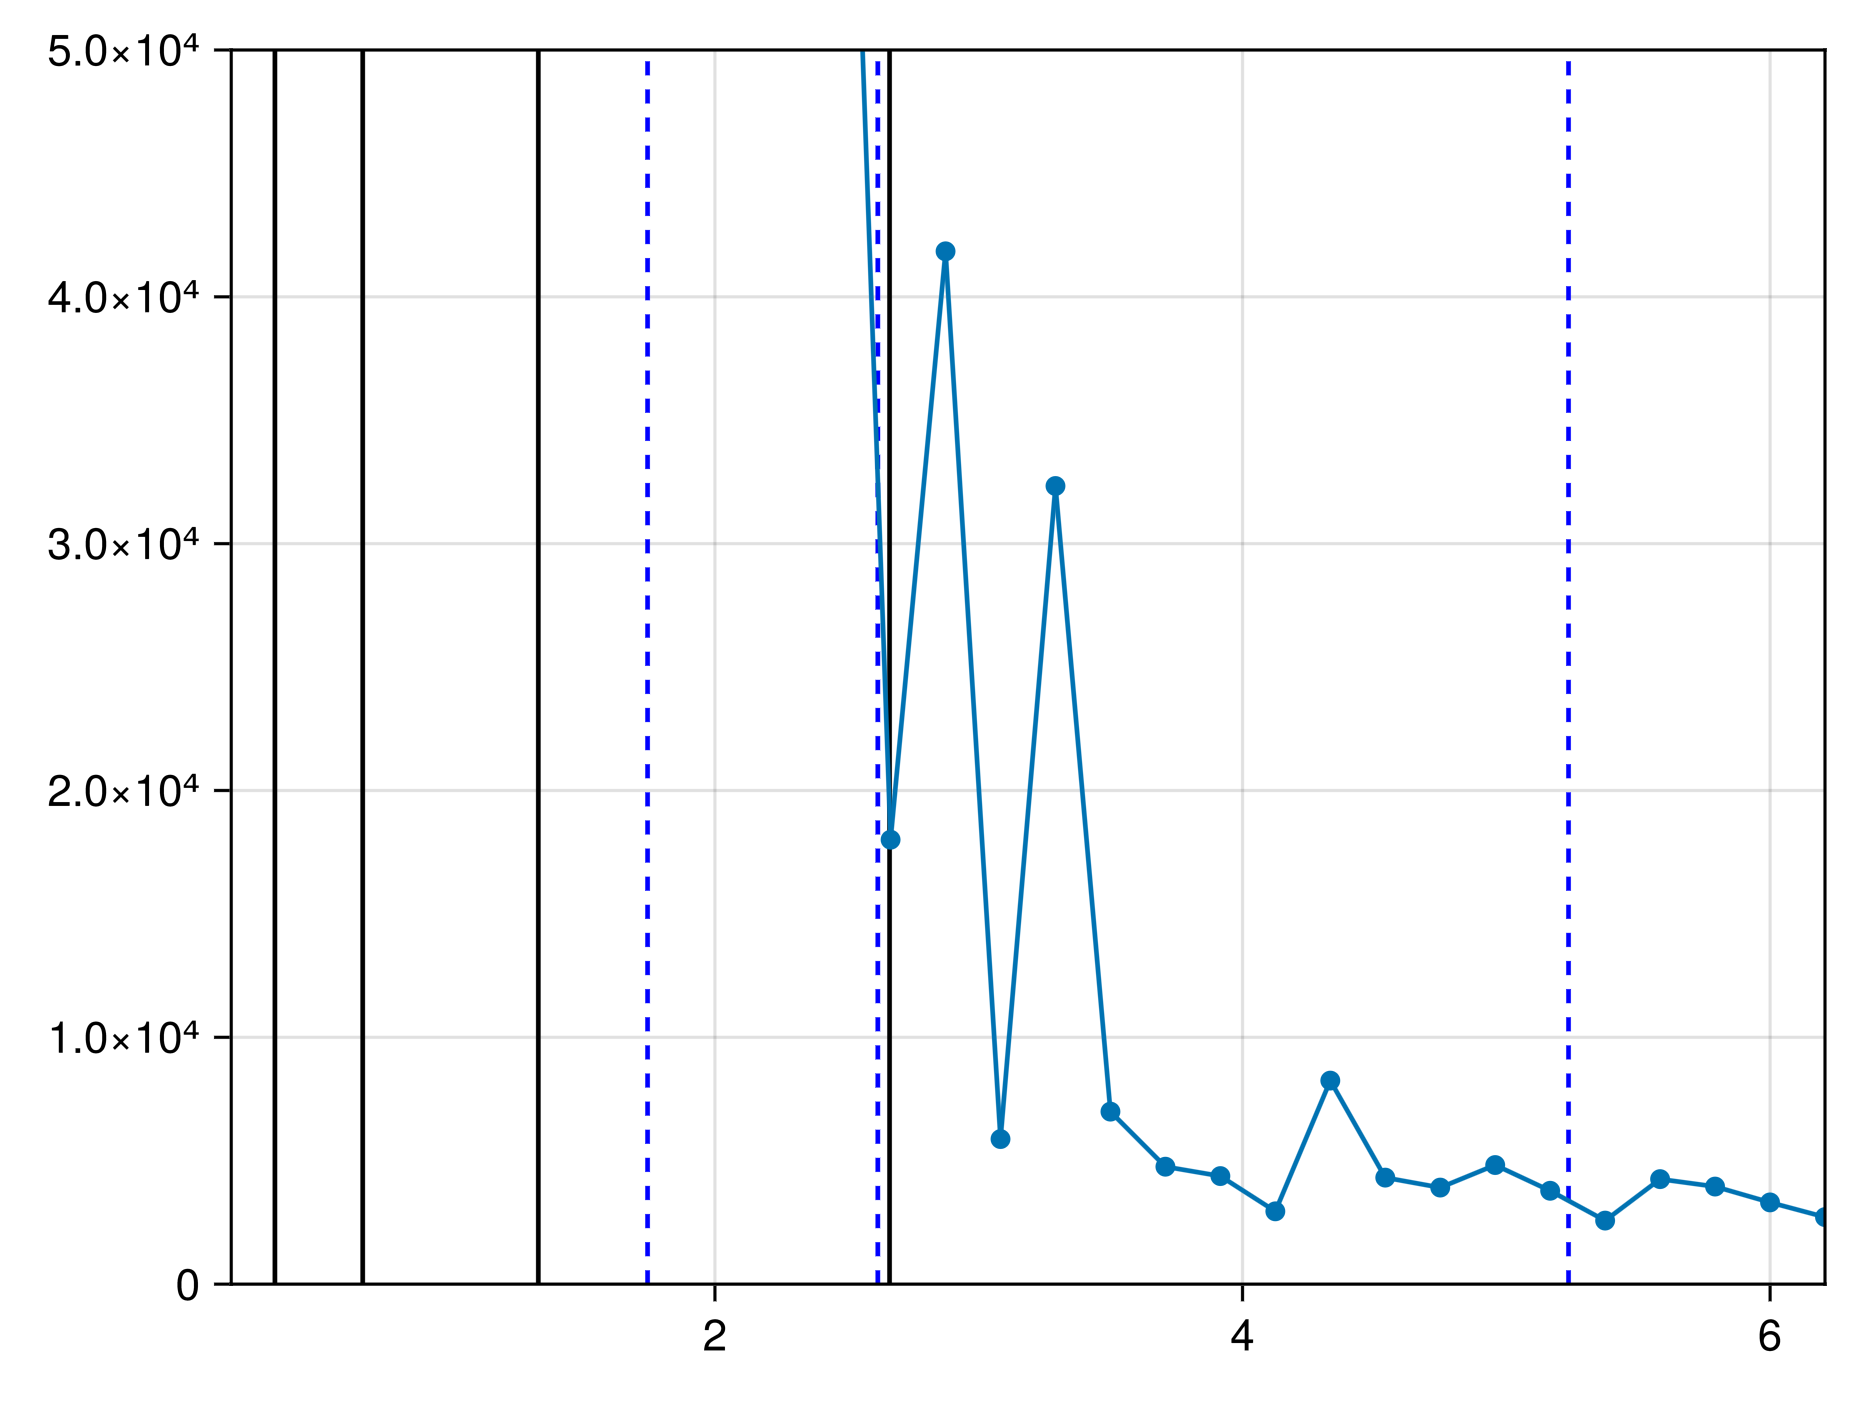
\includegraphics[width=0.9\textwidth]{../Figures/may8/fig_SqCorreccion3A_phi5_d_zoom1_1to.png}
    \caption{Tiempo inicial. 
        Factor de estructura con la corrección. \(\phi=5\%\). 
    Las líneas verticales punteadas en azúl están ubicadas en \(|\vec{q}|=2\pi/1.2,~|\vec{q}|=2\pi/(2\cdot1.2),~|\vec{q}|=2\pi/(3\cdot1.2)\).
    Las líneas verticales punteadas en negro están ubicadas en \(|\vec{q}|\in\{2\pi/L,2\pi/L/2,2\pi/L/4,2\pi/L/8,2\pi/L/16\}\).
}
\end{figure}

Cambié el parámetro para calcular distancias en condiciones de frontera periódicas de \(\lambda_f\) a \(\lambda_f/2\).

\section{Reunion con Asesores}

Usar la distancia con respecto al origen de la caja.
No usar la distancia entre partículas.
Definir el dominio del vector de onda en términos de \(q\), no de lambda.

\begin{figure}[ht!]
    \centering
    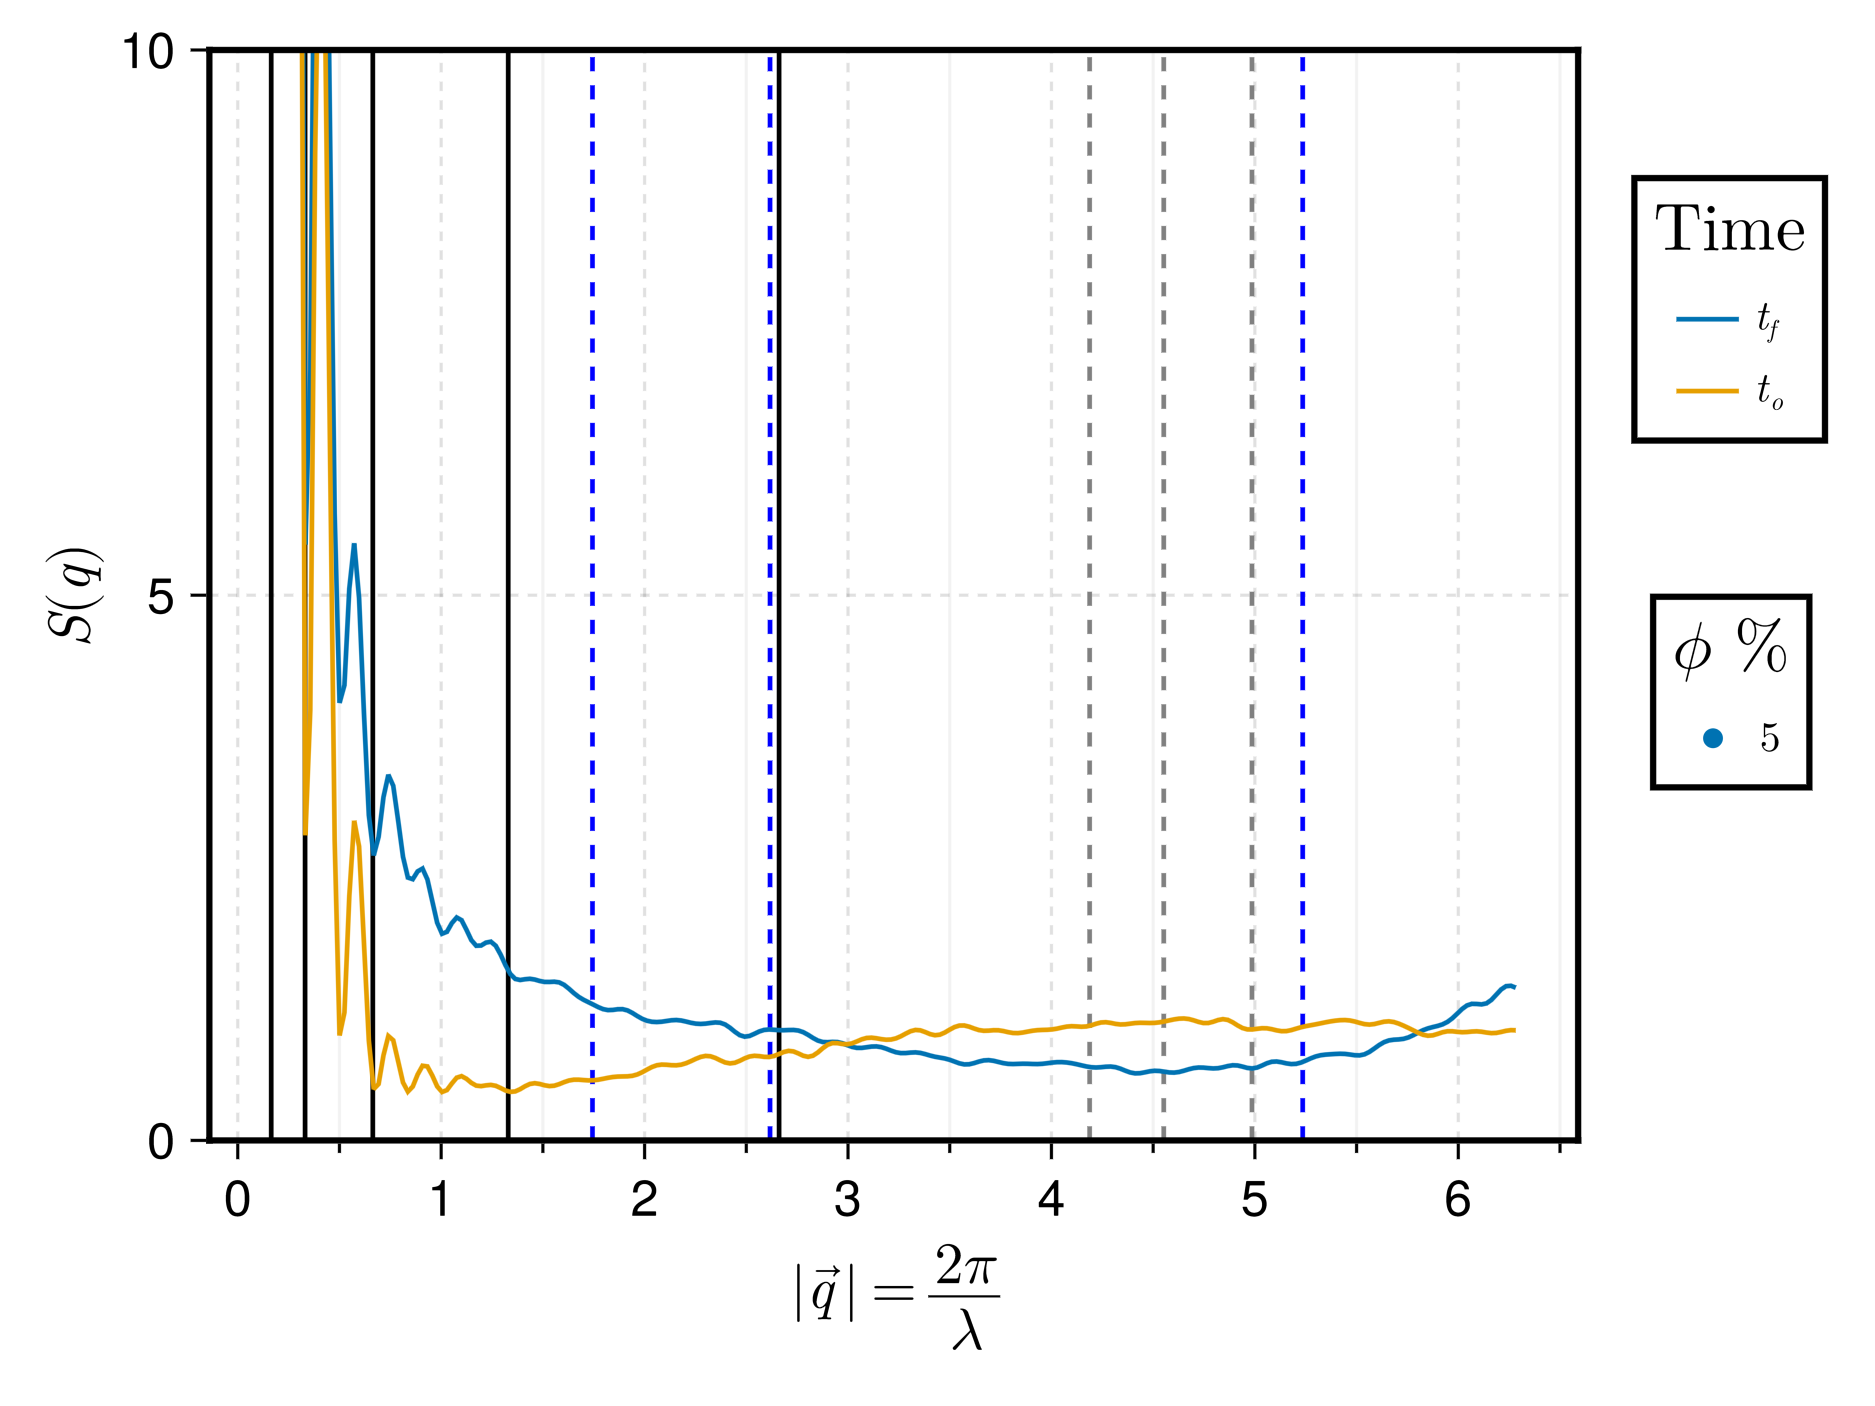
\includegraphics[width=0.9\textwidth]{../Figures/may8/fig_SqCorreccion5_phi5_tfto.png}
    \caption{Factor de estructura usando la distancias con el centro de la caja. \(\phi=5\%\). 
    Las líneas verticales punteadas en azúl están ubicadas en \(|\vec{q}|=2\pi/1.2,~|\vec{q}|=2\pi/(2\cdot1.2),~|\vec{q}|=2\pi/(3\cdot1.2)\).
    Las líneas verticales punteadas en negro están ubicadas en \(|\vec{q}|\in\{2\pi/L,2\pi/L/2,2\pi/L/4,2\pi/L/8,2\pi/L/16\}\).
}
\end{figure}

No me queda muy claro cómo interpretar estás gráficas.
Pero al comparar la gráfica anterior con la siguiente me da un poco de paz que hay diferencias entre las concnetraciones y tiempos iniciales y finales.

Lo que no entiendo mucho es en picos cercanos a \(0\).
Son picos relacionados al tamaño de la caja.
Parece ser que las distancias características están en el orden de \(L/2\) a \(L/8\).

Por el momento, lo que entiendo es que una mayor intensidad en \(|\vec{q}|\) chicas indica que el proceso ayuda a que pase algo a longitudes largas.

\begin{figure}[ht!]
    \centering
    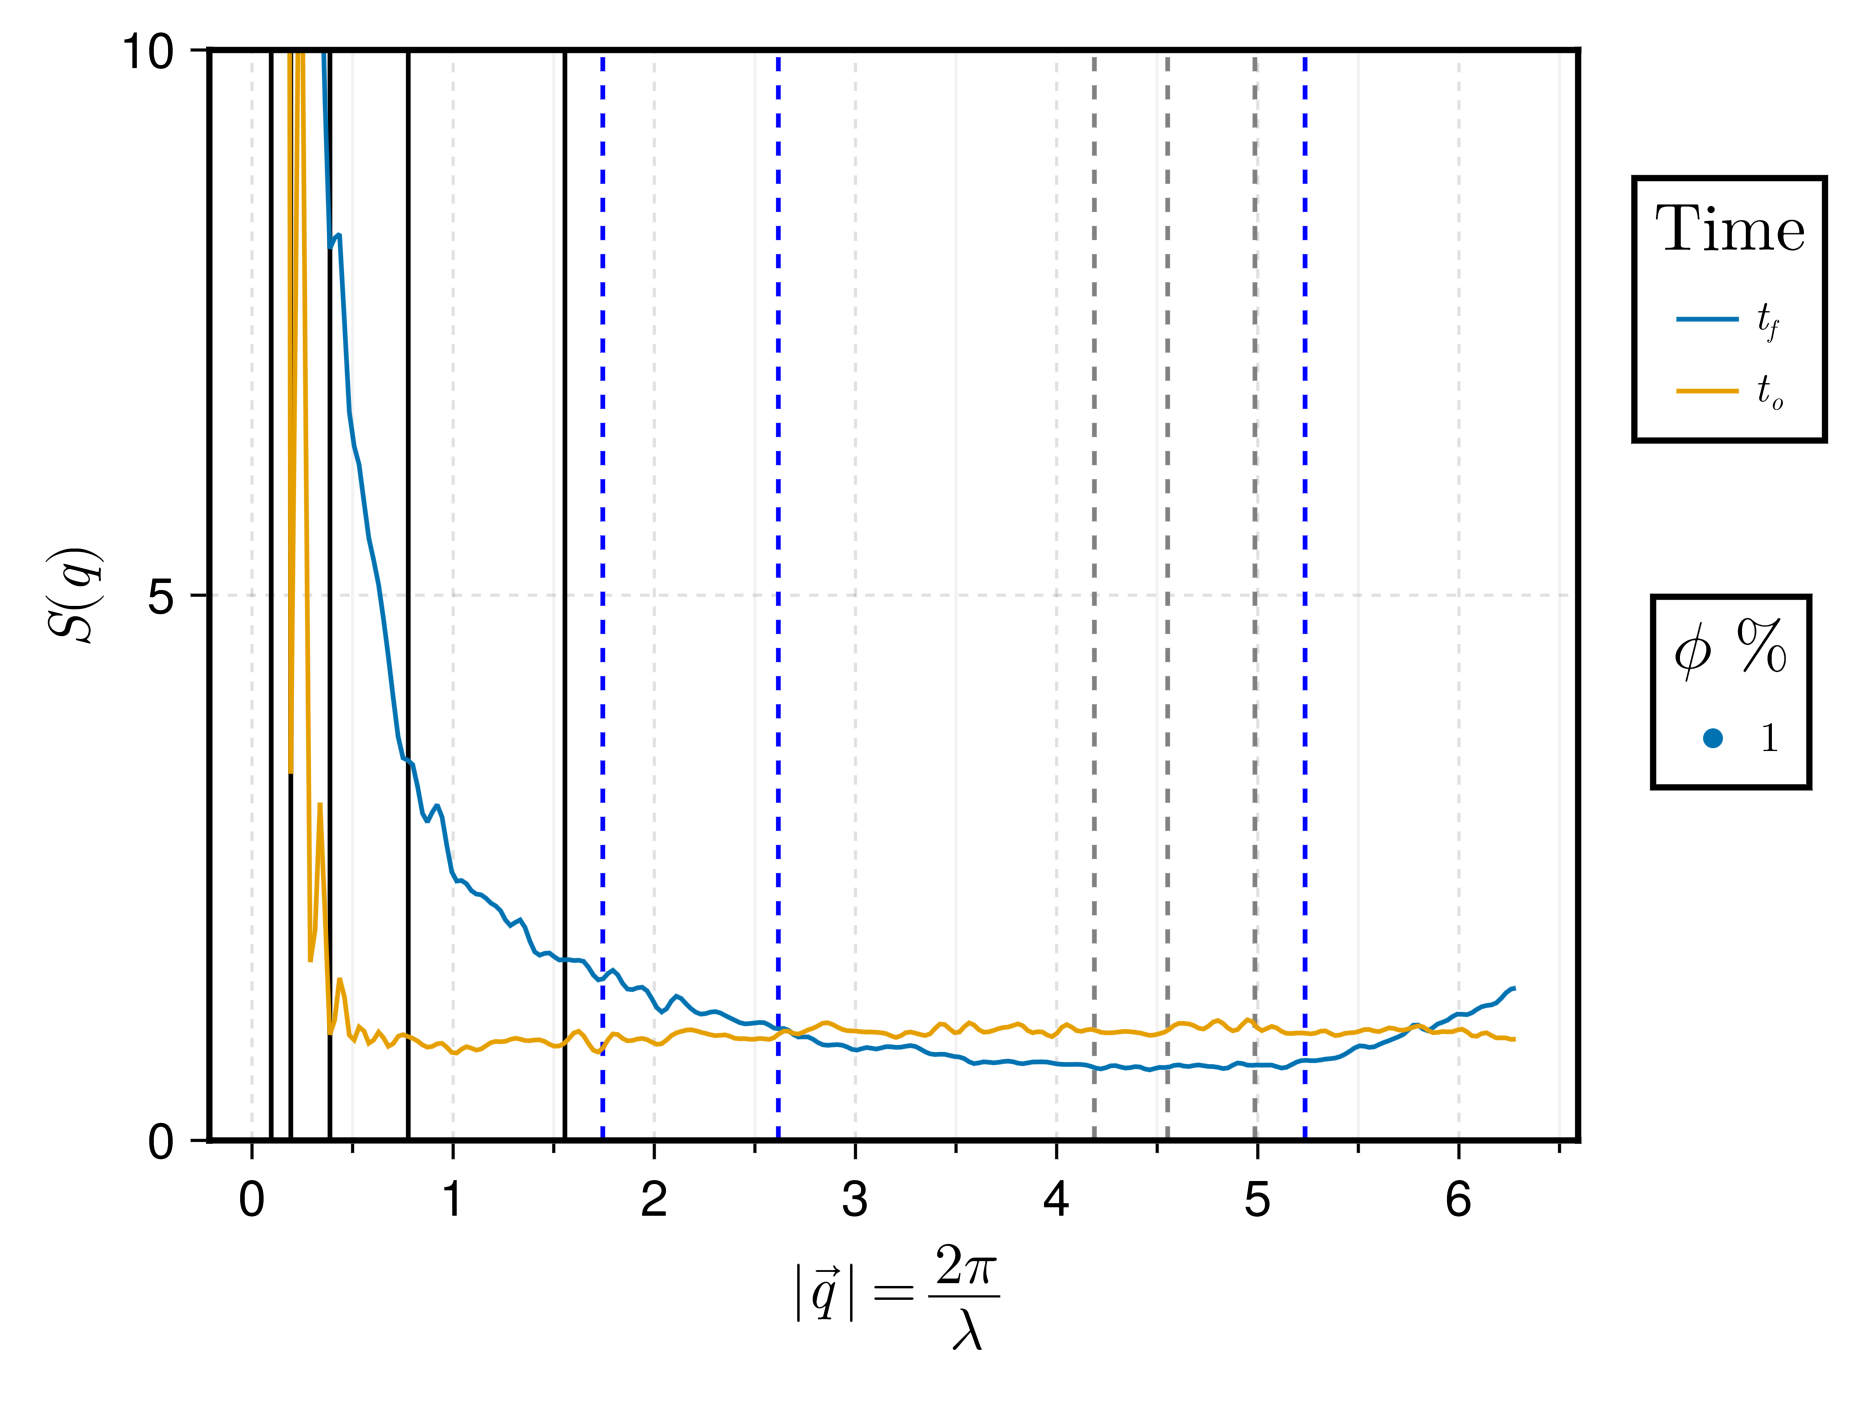
\includegraphics[width=0.9\textwidth]{../Figures/may8/fig_SqCorreccion5_phi1_tfto.png}
    \caption{Factor de estructura usando la distancias con el centro de la caja. \(\phi=5\%\). 
    Las líneas verticales punteadas en azúl están ubicadas en \(|\vec{q}|=2\pi/1.2,~|\vec{q}|=2\pi/(2\cdot1.2),~|\vec{q}|=2\pi/(3\cdot1.2)\).
    Las líneas verticales punteadas en negro están ubicadas en \(|\vec{q}|\in\{2\pi/L,2\pi/L/2,2\pi/L/4,2\pi/L/8,2\pi/L/16\}\).
}
\end{figure}



\end{document}
